\colorlet{chaptergrey}{black}
%\renewcommand*\sectfont{\color{orange}}
\chapter[Discrete dynamical models of stacked dark matter haloes]{Galaxies as potential tracers: \\ Discrete dynamical models of stacked dark matter haloes in IllustrisTNG}
\label{ch:dyn_mod}
\vspace{-5.25in}
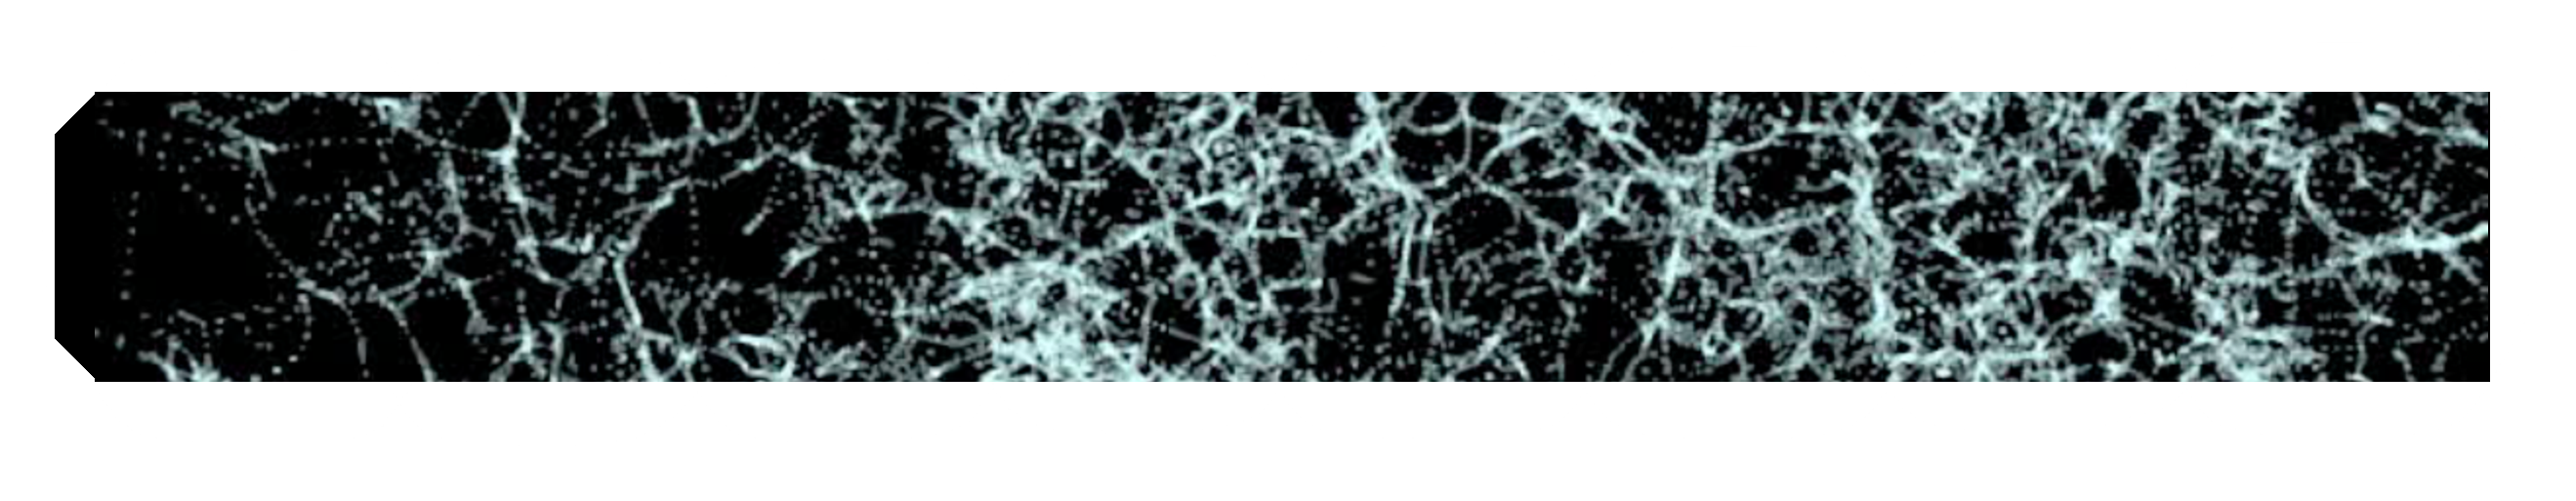
\includegraphics[height=1.39in]{thesis/latex/dyn_mod_files/tngcw_heading.pdf}
\vspace{3in}

%\epigraph{Eat slugs malfoy.}

\section{Introduction}
Numerical simulations show that the anisotropy of the cosmic web imprints distinct signatures in the orbits of particles within dark matter haloes, leading to distinct differences in velocity anisotropy (ratio between velocity moments in tangential and radial directions). On a particle level, the orbits have greater tangential dispersion in haloes within environments of both higher tidal field strength and over- density \citep[e.g.][]{faltenbacher2010, shi2015}. Satellite galaxies also have been shown to trace this anisotropy with orbits becoming more tangentially biased for haloes in closer vicinity to large filamentary structure \citep[][]{garaldi2018}. Observing said velocity anisotropy is tricky in observations without 3D motions.

In this chapter, we demonstrate the relationship between large scale environment and the typical orbits of satellite galaxies in low mass dark matter haloes. Using the cosmological simulation of IllustrisTNG300, we stack low mass haloes in different cosmic web environments (voids, saddle points, and filaments) to recover the difference in velocity anisotropy. We motivate the potential to recover the 3D motions of satellites through a new application of the axisymmetric Jeans equations, and hence, the velocity anisotropy of the environment they trace.

\section{Data}
\subsection{IllustrisTNG300}

\subsection{Galaxy sample} \label{sec:gal_samp}
%Structure in TNG is identified into haloes and subhaloes as follows. Haloes (also referred to as FoF haloes or Groups) are found from a standard friends-of-friends (FoF) algorithm \citep{davis85} with linking length b=0.2. The FoF algorithm is run on the dark matter particles, and the other types (gas, stars, BHs) are attached to the same groups as their nearest DM particle. Each halo is then divided into gravitationally bound subhaloes through the subfind algorithm \citep{springel01}.
To select galaxies in TNG300, we consider all subhaloes at $z=0$ (snapshot 99) containing a minimum stellar mass of $\mathrm{M_{\ast} = 10^{8} M_{\odot}}$ within a 3D aperture of 30 comoving kpc from the subhalo centre \citep[as defined in;][]{pillepich18b}. This corresponds to 564 930 unique galaxies whose positions are used to reconstruct the cosmic web as described in \S\ref{sec:disperse}.

In the context of halo assembly, we are interested in isolating the effects of anisotropy of the cosmic web on low mass dark matter haloes. To this effect, we select all subhaloes that reside in a FoF halo of mass $\mathrm{10^{11.5} M_{\odot} < M_{h} < 10^{12.5} M_{\odot}}$ for use in stacking environments, described in \S\ref{sec:stacking}.

\subsection{DisPerSE}

\begin{figure*}
	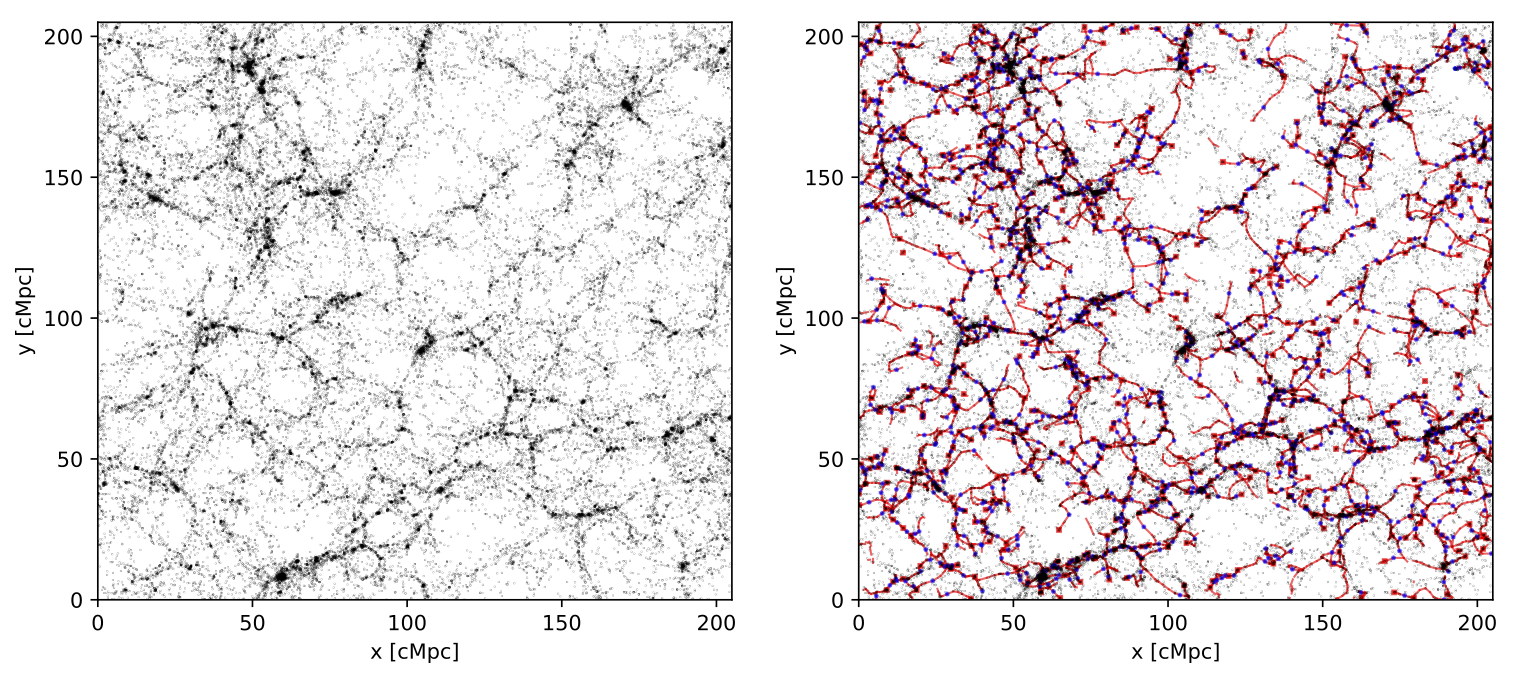
\includegraphics[width=\linewidth]{dyn_mod_files/TNG300-1-SM10-8-slice-galaxy-density-skeleton-comparison.png}
    \caption{Illustration of the filamentary network identified from galaxy positions within a 10 Mpc slice in TNG. The left panel shows the distribution of galaxy ($M_{\ast} > 10^{8}M_{\odot}$) positions within the slice. The right panel shows the same but with filamentary structure overlaid (red lines). Critical points are also shown such as nodes (red squares) and saddle points (blue stars) highlighting the ensemble which the skeleton connects.}
    \label{fig:disperse_TNG300}
\end{figure*}


\subsection{Cosmic web distances}
\red{COPY AND PASTE FROM DUCKWORTH+19}
Having constructed a skeleton of the cosmic web, a galaxy's environment can be described by finding its vicinity to various features of the skeleton. The cosmic web comprises of low density `void' regions which are enclosed by `walls' of structure which become filaments at points of intersection. The gravitational potential of the filaments dictate the flow of the matter, which at the point of intersection, feed high density regions interpreted as `nodes'. Along the filament, saddle points remain as minima between the flows towards nodes. Saddle points are subdivided into 2-saddles and 1-saddles corresponding to the dimensionality of collapse. We take 2-saddles as our environment of interest corresponding to one dimension of recession along the filament, while accretion continues in any direction perpendicular. 

The distance to the nearest filamentary point, $D_{skel}$, is first found for each galaxy. To then consider the influence of the nearest node, the distance from this impact point along the filament to the node (saddle) is also computed, $D_{node}$ ($D_{1-saddle}$,$D_{2-saddle}$). Finally the distance to the nearest wall, $D_{wall}$, can then be found. 

\subsection{Stacking of cosmic web environments} \label{sec:stacking}
In order to stack dark matter potentials and their tracers for the purpose of dynamical modelling, we must be careful about orientation, scaling and effects resulting due to the proximity of other environments. We stack three different environments; filaments, 2-saddles and voids. 

For each environment we select all galaxies in FoF haloes with $\mathrm{10^{11.5} M_{\odot} < M_{h} < 10^{12.5} M_{\odot}}$. To remove effects due to the proximity of other environments, we take all those within the following conservative selections as shown in Table \ref{tab:stacking}. 

\begin{table}
\centering
\begin{tabular}{|l|c|c|c|}
\hline
& Filament & 2-saddle & Void \\ \hline
$D_{node}$ & > 2 Mpc & > 2 Mpc & > 5 Mpc \\
$D_{skel}$ & < 0.5 Mpc  & - - & > 5 Mpc \\
$D_{2-saddle}$ & > 1 Mpc & < 0.75 Mpc & > 5 Mpc \\
Number of galaxies: & 8071 & 941 & 2246 \\
\hline
\end{tabular}
\caption{Selection criteria for stacks in three different environments; filaments, 2-saddle points and voids. Each row shows the distance cut used to select an environment apart from the final row which shows the total number of galaxies selected.}
\label{tab:stacking}
\end{table}

To construct a reliable dynamical model, all tracers should reside in gravitational potentials that are consistent in overall mass and scale. For every FoF halo that contains a galaxy to be stacked we take the density profile and scale it according to the characteristic group scale as defined by $R_{200}$ (comoving radius of a sphere centered on the FoF halo whose mean density is 200 times the critical density of the Universe). The magnitude of the density profile is scaled according to the total mass contained in the FoF halo and then combined so that each stacked density profile contributes equally to the final profile. The stacked FoF halo density profile is finally scaled so that its total mass is equal to the median for the stacked population. We then convert the final density profile to the gravitational potential as described in \ref{sec:grav_pot}.

Each tracer position and velocity is also scaled by the characteristic group scale of its host FoF halo, $\mathrm{R_{200}}$. \red{Should velocity be scaled according to mass or is this accounted for by the scale?}. 

A natural assumption of our Jeans formalism is symmetry around the principal axis of rotation, so it is important to retain directionality while stacking tracers and potentials. In the instance of 2-saddle points and filaments, we use the direction of the nearest filament segment (from 2-saddle to node) to stack along. For those stacked in the void environments we use the direction of the angular momentum vector for the central subhalo. \red{Do this from stellar only?, do this for whole FoF halo? - check correlation?}

\subsection{Velocity anisotropy}
On a particle level, the orbits within FoF haloes have been shown to be dependent on large scale environment. \citet{faltenbacher2010} used an implementation of the Tree-PM N-body code GADGET2 on-top of the Millenium simulation. They examine the correlation between clustering and halo properties such as shape, concentration, spin, shape of the velocity ellipsoid and velocity anisotropy. The velocity anisotropy parameter is defined as
\begin{equation} \label{eq:vel_ani_sigma}
\mathrm{\beta_{\sigma}(r) = 1 - \frac{\sigma_t^2(r)}{\sigma_r^2(r)} }
\end{equation}
where $\sigma_r^2(r)$ and $\sigma_t^2(r)$ denote the radial and tangential velocity dispersions. Note that this equation can also be presented as an average for a halo. 

They determine that $\beta_{\sigma}$ is most tightly correlated with the clustering strength, with halos of low velocity anisotropy being more highly clustered and the opposite holding true for haloes with strongly radially biased velocities. 

A possible explanation for more highly clustered haloes exhibiting a relatively larger tangential velocity dispersion is that the impact parameters of the merging sub-haloes are larger due to far more gravitational interactions a short time before accretion. This would lead to a greater dispersion of tangential velocities corresponding to a lower velocity anisotropy. On the other hand, in less clustered regions the gravitational field is dominated by the halo itself naturally leading to more radial in-fall. 

Further, velocity anisotropy has also been decomposed as a function of tidal environment. \cite{shi2015} investigate how halo dynamical properties are related to their formation histories and hence the tidal environment in which they reside. They demonstrate a clear correlation between $\beta_{\sigma}$ and the first eigenvalue of the tidal tensor (i.e. tidal field strength) for both low mass and high mass haloes. As tidal field strength increases, $\beta_{\sigma}$ decreases, showing that again there is a greater dispersion in tangential orbits. 

In the right panel of Figure \ref{fig:beta_stack}, we show $\beta_{\sigma}$ calculated directly from the satellite tracers in our void (red, dotted), filament (black, dot-dashed) and 2-saddle (green, solid) stacks. Within 0.1 Mpc of the halo centre, $\beta_{\sigma}$ is roughly consistent between environments. Above 0.1 Mpc, however, there is a clear difference between the three environments with 2-saddles exhibiting a relatively larger tangential velocity dispersion and voids displaying more isotropic orbits. The gray box inlaid in the panel shows $\overline{\beta_{\sigma}}$ calculated from all satellite tracers. The clear difference between voids, filaments and 2-saddles dictates that trends previously shown on a particle level can be recovered from satellites as tracers. 

\begin{figure*}
	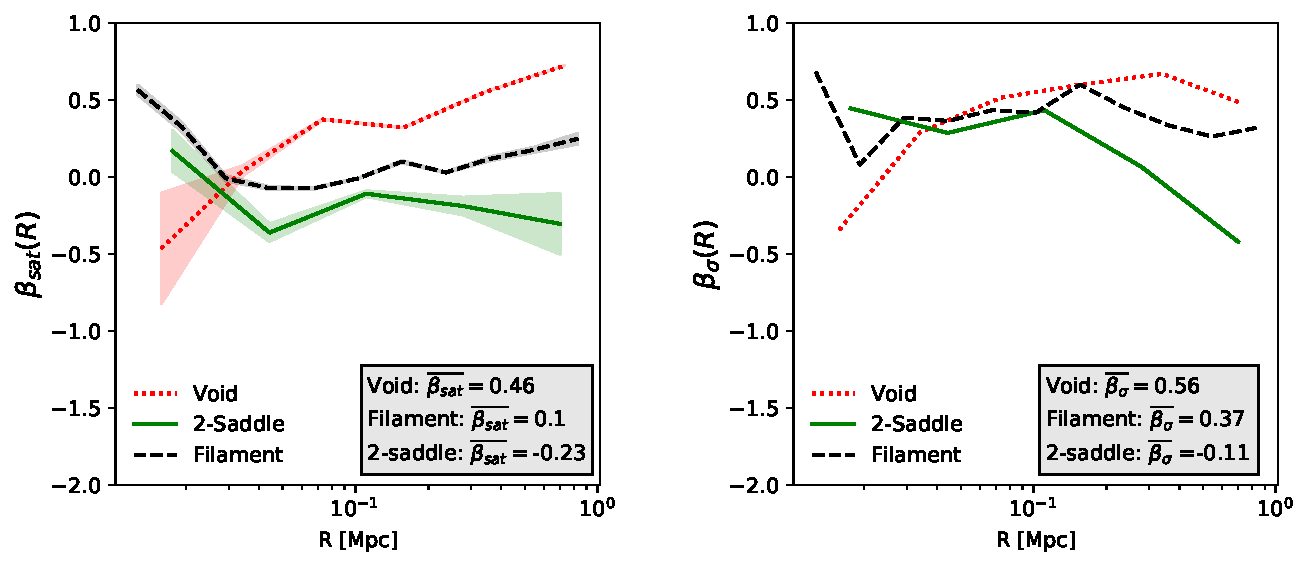
\includegraphics[width=\linewidth]{thesis/latex/dyn_mod_files/disperse_beta_paper.pdf}
    \caption{Velocity anisotropy profiles found from satellite galaxies in the void (red, dotted), filament (black, dot-dashed) and 2-saddle (green, solid) stacks. The left (right) panel corresponds to $\beta_{sat}$ ($\beta_{\sigma}$) with the shaded regions showing error on the mean. The average value for all satellites in each stack is shown in the grey box. For both $\beta_{sat}$ and $\beta_{\sigma}$, there is a clear distinction in orbital anisotropy between environments which increases with radii.}
    \label{fig:beta_stack}
\end{figure*}

The orbits of satellite galaxies in the context of the cosmic web has been previously considered in a set of zoom N-body and hydrodynamical simulations \citep{ZOMGiii}. They define the satellite anisotropy parameter as
\begin{equation}
\beta_{sat}(r) = 1 - \frac{v_{t}^2(r)}{v_{r}^{2}(r)} 
\end{equation}
where $v_{t}(r)$ and $v_{r}(r)$ denote the radial and tangential velocities. They follow seven galaxy sized haloes ($M_{h} \sim 10^{11} M_{\odot}$) which are classified as `stalled' or accreting corresponding to the time at which their final mass becomes stable. The accreting haloes correspond with \green{voids?} nodes of the cosmic web and are fed isotropically by radial infall of matter along filaments. Conversely `stalled' haloes are embedded in prominent filaments of the large-scale structure. They find that the satellite anisotropy parameter at $z = 0$ is positive for accreting haloes and negative for stalled haloes showing that orbits become more tangentially biased (both in magnitude and dispersion) when low mass haloes are closer to large filamentary structure. 

In the left panel of Figure \ref{fig:beta_stack}, we show $\beta_{sat}$ again calculated directly from the satellite tracers in our void (red, dotted), filament (black, dot-dashed) and 2-saddle (green, solid) stacks. We again see a clear distinction between environments in the anisotropy with 2-saddles exhibiting orbits with stronger tangential velocity components at larger radii. The gray box inlaid shows $\overline{\beta_{sat}}$ found from all satellites within the stacks. In-keeping with \citet{ZOMGiii}, we find that the satellite anisotropy becomes more tangentially biased as we more closer to large filamentary structure.

It should be noted that while it is important to retain directionality in stacking for the purpose of dynamical modelling, it has no impact on the direct measures of $\beta_{\sigma}$ and $\beta_{sat}$.